\begin{figure*}[t]
  \centering
  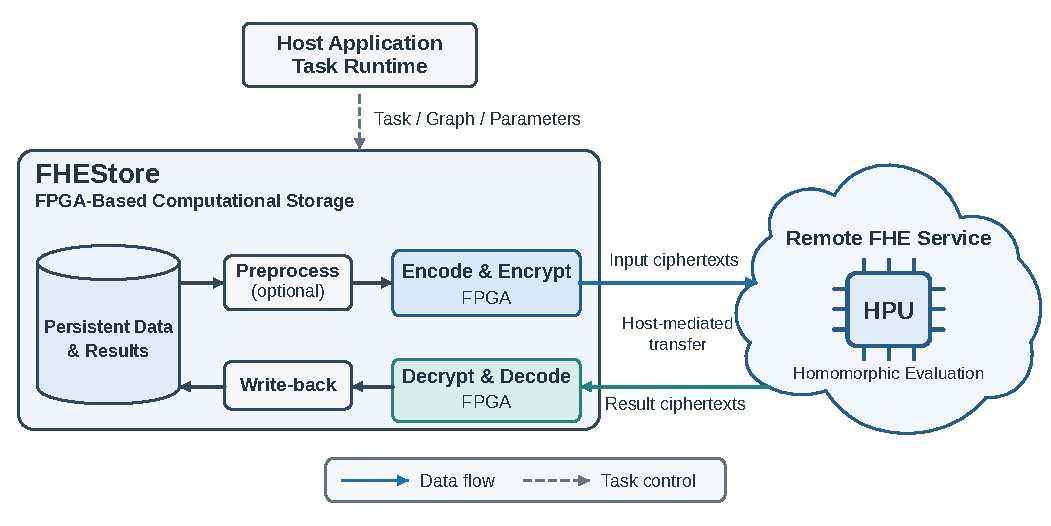
\includegraphics[width=\textwidth]{figures/fhestore-overview-v1/fhestore-overview.pdf}
  \caption{Functional overview of FHEStore. Storage-side input preparation produces ciphertexts for an external FHE service, while the return path decrypts results and writes recovered application data to persistent storage. Solid arrows denote logical data flow; dashed arrows denote host task control. Ciphertext exchange is host-mediated, and record updates may involve host-assisted read--modify--write.}
  \Description{The host application and task runtime configure FHEStore. Its input path connects persistent data to optional preprocessing and FPGA encoding and encryption. Input ciphertexts are transferred through the host to a remote FHE service represented by an HPU. Returned result ciphertexts enter FPGA decryption and decoding, followed by write-back to persistent storage.}
  \label{fig:fhestore-overview}
\end{figure*}
